\chapter{Val av verktyg vid projektdokumentation av Daniel Wassing}
\section{Introduktion}
\label{cha:wassing-introduction}
Projektdokumentation är en kritisk roll för lyckade projekt. Dokumentation behövs i många stadier och alla är väldigt relevanta för projektets framgång. Från att en projektplan och kravspecifikation tas fram och skrivs tills det att en slutrapport med användarhandledning lämnas in så spelar dokumentationen en central roll i projektets arbetsgång och tidsram. 
\\ \\
Hur man skriver dokument lär man sig redan från barnsben och man slutar aldrig lära sig - på universitetet får man fortfarande lära sig hur man skriver akademiskt korrekt. Men när det gäller verktygen för dokumentation så erbjuds det i dagsläget ingen kurs på Linköpings universitet för hur man använder dem, och verktygen spelar en väldigt stor roll i hur framgångsrik dokumentationen är.

\subsection{Motivering}
\label{sec:wassing-motivation}
Allt eftersom mjukvaruindustrin växer så växer även behovet av att dokumentera korrekt och effektivt. Då det kan ta väldigt mycket tid att dokumentera så är det väldigt viktigt att det effektiviseras. Olika projektmedlemmar kan behöva hjälpa till med dokumentation, och då är det viktigt att alla kan jobba parallellt utan att olika data går förlorade eller skrivs över. Bra dokumentation kan uppnås på flera sätt, men studenter på utbildningarna för datateknik och mjukvaruteknik vid Linköpings universitet får inte någon utbildning inom olika dokumentationsmetoder. Därför är det svårt, om inte omöjligt, att avgöra vad man bör använda för verktyg för att vara så tidseffektiv som möjligt vid dokumentation av projekt. Olika verktyg medför olika för- och nackdelar samt utmaningar.

\subsection{Målsättning}
\label{sec:wassing-aim}
Den här rapporten ämnar att tydliggöra vilka för- och nackdelar olika verktyg medför när man dokumenterar för ett projekt, mer specifikt vad man kan spara tid på och vilka fördelar man kan få i slutdokumentationen. Rapporten ämnar även att belysa vilka utmaningar grupper kan ställas inför när de väljer hur de ska dokumentera sina projekt och vad de skulle kunna basera sina val på.

\subsection{Frågeställningar}
\label{sec:wassing-research-questions}
Den största utmaningen för valet av verktyg i projektdokumentation för kandidatprojektet i programvaruutveckling är i startläget gruppens kunskap, då ingen vet vad som är tidseffektivast. Nya verktyg kan ta väldigt mycket tid att lära sig, och det är ett stort steg från att ha fått grepp om deras grundläggande funktioner och attribut tills det att man arbetar effektivt med dem. Studiens frågeställning är således: \\

\textbf{"Vilka kriterier är viktiga för ett dokumentationsverktyg i ett kandidatarbete?"} \\ \\
För att bryta upp ovanstående frågeställning så kommer två aspekter besvaras noggrannare:
\begin{enumerate}
\item \textit{Vilka uppenbara för- och nackdelar medför de verktyg som finns tillgängliga för att dokumentera i ett projektarbete?}
\item \textit{Vilka kriterier väger tyngst vid valet av verktyg att dokumentera med?}
\end{enumerate}

\subsection{Avgränsningar}
\label{sec:wassing-delimitations}
Studien i sin helhet baseras på kandidatarbetet som utfördes av grupp två i kursen TDDD96 våren 2017, intervjuer som hållits med några medlemmar ur slumpvis utvalda grupper från samma kurs, samt de referenser som nämns i det här dokumentet.

\section{Bakgrund}
När gruppen sattes samman i början av kursen TDDD96 under vårterminen 2017 så fanns det inte mycket erfarenhet av dokumentation på en akademisk nivå i gruppen. Det fanns väldigt få medlemmar som tidigare hade jobbat med typsättningsprogram och det saknades bra beslutsunderlag för hur gruppen skulle jobba framöver. Det var väldigt stora beslut som behövde fattas på kort tid, beslut som skulle visa sig ha både positiva och negativa konsekvenser för resten av arbetet under hela projektets gång. Hade gruppen haft mer information om verktygen som fanns tillgängliga hade ett mer enat beslut kunnat tas där fler medlemmar haft möjlighet att diskutera och resonera. Gruppens dokumentansvarige började utbilda sig inom valda verktyg för att hjälpa sina gruppmedlemmar komma igång med dokumentationen så fort som möjligt.

\section{Teori}
\label{cha:wassing-theory}
De fakta som presenteras i denna rapport är hämtade från \textit{Documentation in System Development: A significant Criterion for Project Success} \cite{docsystemdev}, \textit{Collaborating with ShareLaTeX and git} \cite{website:sharelatex_with_git} samt \textit{How SciGit and other collaborative editing/version control services are different} \cite{website:scigit_blog}. \\
Fakta presenteras även från intervjuer som har skett under projektets gång.
\\ \\
Nedan presenteras ett flertal av de olika verktyg som tillfrågade personer från olika grupper har använt sig av. Dessa verktyg är de som kommer att behandlas i denna rapport.

\subsection{LaTeX}
\LaTeX (Lamport TeX) är ett så kallat \textit{märkspråk} för att producera dokument, precis som \textit{HTML} är ett märkspråk för webbprogrammering. LaTeX skapades av \textbf{Leslie Lamport}. Den senaste versionen heter LaTeX2e och släpptes 1994, med mindre uppgraderingar som släpps ungefär varje halvår.\cite{website:latex_update_release}
\\ \\
LaTeX bygger på typsättningssystemet \textit{TeX} som utvecklades av \textbf{Donald Knuth} under 1970 och 1980-talet. Språkdefinitionen blev fastställd under 1985 \cite{the_tex_book}.
\\ \\
LaTeX används i dag främst i vetenskapliga kretsar, framför allt inom områdena matematik, fysik och datavetenskap. Det omfattar dokumentstilar för artiklar, böcker, brev, presentationer med mera samt stöd för referenser och automatisk numrering av avsnitt och ekvationer. LaTeX är förmodligen det vanligaste sättet att utnyttja grundprogrammet TeX då det finns väldigt mycket funktionalitet färdig från början, utan att man behöver importera eller använda annan mjukvara. LaTeX kan generera en mängd dokumentformat, den vanligaste är PDF.

\subsection{Git}
\label{sec:wassing-git}
\textit{Git} är ett versionshanteringsprogram som skapades 2005 av \textbf{Linus Torvalds} för att hantera källkod till Linuxkärnan. \cite{website:git} \cite{website:git_version_control} Git kan jämföras med \textit{CVS} eller \textit{Subversion} som också är versionshanteringssystem. Till skillnad från de andra två är däremot Git de-centraliserat, vilket betyder att det inte finns ett mästerarkiv som alltid har den senaste versionen av ändringar.\cite{website:centralized_version_control} CVS och Subversion tas ej upp här då ingen tillfrågad grupp har använt sig av de systemen.
\\ \\
Git är främst tänkt för filer med oformaterad text, men har på senare tid fått utökat stöd för binära filer såsom Microsoft Word dokument. Detta kräver dock tilläggsprogram som ofta bara konverterar binära filer till oformaterad text \cite{website:using_git_with_word}. Användningen av olika tilläggsprogram gör ofta att Git inte är ett alternativ när man jobbar med binära filer. Mer om det i avsnitt \ref{cha:wassing-discussion}.

\subsection{Google Drive}
\textit{Google Drive}, även tidigare känt som \textit{Google Docs}, är en molntjänst som tillhandahålls konstnadsfritt av Google.\cite{website:googledrive} Genom molntjänsten kan användare redigera samma dokument samtidigt. Dessutom kan även andra filer laddas upp och delas. Google Drive kräver en internetanslutning för att användare ska kunna komma åt dokumenten, men är oberoende av plattform då Google Drive exekveras i webbläsaren. Det finns möjlighet att exportera dokument som skrivs i Google Drive till andra format, bland annat PDF.

\subsection{ShareLaTeX}
\textit{ShareLaTeX} är också en molntjänst för fildelning och kollaboration, fast med att skriva dokument i LaTeX som enda funktion.\cite{website:sharelatex} ShareLaTeX  är likt Google Drive plattformsoberoende och körs direkt i webbläsaren. Det finns en enorm support för olika LaTeX och TeX bibliotek och tilläggsprogram, vilka alla kan kallas på direkt i dokumenten när man skriver online utan att vidare arbete behöver utföras. ShareLaTeX har även ett begränsat stöd för att arbeta med Git sedan hösten 2015.\cite{website:sharelatex_git_sync}
\\ \\
Likt LaTeX så används ShareLaTeX primärt för att skapa PDF-filer av hög kvalitet.

\subsection{Microsoft Office}
\textit{Microsoft Office} är en paketlösning från Microsoft som innehåller de populära programmen Word, Excel och Powerpoint med flera. Officepaketet är en köpvara, men studenter på Linköpings universitet kan få det gratis genom internetportalen \textit{Lisam}. \cite{website:liu_office_package} Word tillåter skapande av dokument genom ett stort antal funktioner. Word har däremot ingen inbyggd delningsfunktion, vilket gör att inte mer än en person åt gången kan jobba med ett dokument.
\\ \\
I senare versioner av Office så finns det även möjligheten att exportera till andra filformat än de typiska som mjukvara i Office använder sig av (.doc, .xls och .ppt). 
Microsoft Office används fortfarande flitigt inom industrin. Det erbjuds fortfarande utbildning i Microsoft Office i grundskolan och gymnasiet i dag.

\subsection{WYSIWYG}
WYSIWYG (\textit{What you see is what you get}) är när man dokumenterar med fokus på ordbehandling, vilket gör att det som skrivs är det som fås i slutändan. WYSIWYG går ut på att man producerar ren text och sedan behandlar den med verktyg för formatering, där verktygen varierar beroende på vilket program man använder. Exempel på mjukvara som använder sig av WYSIWYG är Microsoft Office Word och Google Drive.

\section{Metod}
\label{cha:wassing-method}
För att få svar på de frågor som togs upp i avsnitt \ref{sec:wassing-research-questions} så intervjuades ett antal projektmedlemmar ur olika grupper under andra halvan av projekttiden. Deltagarna valdes ut slumpmässigt beroende på vilka som var tillgängliga och samarbetsvilliga. En träff bestämdes för varje deltagare. På träffen hölls en intervju där deltagaren fick svara på frågor. Alla deltagare fick svara på samma frågor. Frågorna hade i förväg utarbetats för att tangera frågeställningarna men även generera öppna svar, då det ansågs vara av intresse att få reda på hur olika grupper hade tacklat olika problem på vägen. Frågorna som ställdes återges nedan: %möjligen ändra till appendix senare
\begin{itemize}
\item{Med vilka verktyg dokumenterar din grupp?}
\item{Hur togs besluten av val av verktyg för dokumentation?}
\item{Vilka fördelar med dessa verktyg ser du/ni?}
\item{Vilka nackdelar ser du/ni?}
\item{Hade ni kunnat föreställa er att använda andra verktyg?}
\item{Med tanke på att kandidatarbetet behandlar väldigt mycket dokumentation så kan det vara bra att ha mallar att utgå ifrån (inte minst för slutrapporten). Det finns mallar för kandidatuppsatser tillgängliga. Har dessa mallar varit användbara för er? Har de varit applicerbara?}
\end{itemize}
Det som sades på intervjuerna antecknades och renskrevs för tydlighet. Svaren har sammanställts utefter vilka verktyg som deltagarnas grupper valt och tas upp i avsnitt \ref{cha:wassing-results}.
\\ \\
Till grund för diskussionen som presenteras i avsnitt \ref{cha:wassing-discussion} ligger även konferensbidraget \textit{Documentation in Systems Development: A Significant Criterion for Project
Success} \cite{docsystemdev}. %kanske mer här sen men det är fuckat att hitta vettiga källor

\section{Resultat}
\label{cha:wassing-results}
I den här delen presenteras resultaten från intervjuerna som hållits med deltagare i kursen TDDD96, våren 2017. För intervjuernas struktur, se avsnitt \ref{cha:wassing-method}.

\subsection{LaTeX}
\label{sec:wassing-latex}
De flesta av de tillfrågade deltagarnas grupper hade använt sig av typsättningsspråket LaTeX. LaTeX upplevdes ha en exponentiellt ökande grad av nytta. Det kunde vara trögt att komma igång, men takten att producera nya och bättre dokument ökade ju längre projektet framskred. Trenden var att bara en minoritet någonsin hade använt LaTeX i varje grupp, om någon hade gjort det över huvud taget. Det handlade ofta om bara en eller två personer som var bekanta med det sedan tidigare. Det var nästan alltid en person med tidigare kunskap i LaTeX som blev utsedd att vara dokumentansvarig.

\subsubsection{Fördelar med LaTeX}
Fördelarna var många, menade de som använt det. Tillfrågade personer menade att programmerare har ofta en tendens att inte vilja använda muspekaren och bara knappa på tangentbordet. Detta är något som LaTeX tillgodoser då det av ren märkspråksnatur handlar om att skriva kod och text. Grafiska representationer för infogande av bilder och dylikt existerar inte, utan allt löses genom ren kodskrivning. LaTeX ger möjligheten att göra stora övergripande ändringar av enorma dokument med ändring av bara några enstaka rader kod och ger skribenten full kontroll. LaTeX ger även möjligheten att dela upp arbetet med ett dokument i flera filer. Flera filer gör systemet mer modulärt, vilket innebär att det blir mycket smidigare att ändra i, speciellt då flera personer arbetar samtidigt.

\subsubsection{Nackdelar med LaTeX}
Den uppenbara nackdelen som nämndes var inlärningskurvan. LaTeX har väldigt många möjligheter, men som vilket annat programmeringsspråk som helst så krävdes det tid innan medlemmarna var införstådda med den syntax som krävdes för produktion av dokument. LaTeX är ett typsättningssystem och inte ett ordbehandlingssytem, vilket leder till att det man skriver inte direkt reflekterar det man får i slutändan, till skillnad från WYSIWYG. Då tidsbrist ofta var ett problem blev inlärningskurvan en ganska central punkt att ta ställning till vid valet av dokumentationsverktyg. Mer om det i avsnitt \ref{cha:wassing-discussion}. 

\subsection{Git}
\label{sec:wassing-gitresults}
Alla tillfrågade grupper hade använt sig av Git, dock inte alltid för dokumentationen. Versionshanteringssystem såsom Git är centralt för utveckling av mjukvara, men av intervjuerna framgick det att det inte är lika erkänt för dokumentation. För- och nackdelar som redovisas nedan är sett helt ur ett dokumentationsperspektiv, ej utveckling.
\\ \\
En stor del av de tillfrågade förklarade att de använde Git vid dokumentation utöver utveckling. Det visade sig vara användbart att kunna versionshantera även dokument då individer kan råka radera eller ändra på fel ställe i dokument.

\subsubsection{Fördelar med Git}
De som använde Git för dokumentation citerade versionshanteringens egenskaper: Git tillåter användare att hålla reda på historik och förändringar i dokument, samt gör det möjligt att backa tillbaka i tiden eller att spåra vem som har gjort vad. Detta var till nytta för samtliga som versionshanterade sina dokument med Git. Se avsnitt \ref{sec:wassing-git} för information om hur versionshantering går till.

\subsubsection{Nackdelar med Git}
Två nackdelar nämndes, dessa var inlärningskurvan och sammanslagningskonflikter.
\\ \\
Versionshantering har som det mesta annat en inlärningskurva. För att komma igång med Git så tillhandahölls interna guider och utbildning från ansvariga personer i grupperna.
\\ \\
Sammanslagningskonflikter är när två eller flera personer utför ändringar på samma ställe i ett dokument och alla som vill uppdatera dokumentet efter den första personen får en konflikt från Git. 
Dokument som fick konflikter behövde granskas för att lösa konflikterna manuellt. För en oerfaren person kunde sammanslagningskonflikter ses som något jobbigt då personen inte visste vad som skulle stå kvar och tas bort. Personen som påpekade att sammanslagningskonflikter var en nackdel medgav dock senare att de finns till för att hjälpa. De sågs bara som något nytt och otäckt, vilket gav ogrundad rädsla.

\subsection{Google Drive}
\label{sec:wassing-googledrive}
Alla tillfrågade förklarade att deras grupper hade gemensamma Drive-kataloger där dokumentation sparades. Utsträckningen av vilken dokumentation som sparades varierade, vissa valde att dokumentera allt i Google Drive, medans andra nöjde sig med gruppdokument som inte låg i kunds intresse att se. Sådana dokument var till exempel riktlinjer för hur gruppmedlemmarna gjorde olika saker, mötesprotokoll och rapporter.

\subsubsection{Fördelar med Google Drive}
\label{subsec:wassing-googledrive-pros}
Fördelarna var många, menade de tillfrågade. Drive körs i webbläsaren och är därför plattformsoberoende. Tillgång till internet var inget problem på campus eller vid arbete hemifrån så det ansågs inte vara en begränsning.
\\ \\
Systemet använder sig av WYSIWYG-metodiken. Google Drive ansågs vara pedagogiskt och det fanns en stor hjälpdatabas som enkelt kunde hittas genom sökning med godtycklig sökmotor om frågor uppstod. Drive tillät dessutom flera människor att jobba samtidigt på ett och samma dokument. Stöd för arbete offline fanns om internet inte fanns att tillgå, men det fungerade dock bara om dokumentet som jobbades på redan fanns lagrat lokalt i webbläsaren.

\subsubsection{Nackdelar med Google Drive}
Det nämndes inte mycket nackdelar med Google Drive förutom att det krävde internet. Dock togs det upp att Google Drive hade mindre funktionalitet för skapande av högklassiga dokument än vad exempelvis Microsoft Office hade. Office hade mer användarvänlighet, ett enkelt användargränssnitt och en stor mängd mallar att använda vid skapande av dokument som Google Drive saknade.

\subsection{ShareLaTeX}
\label{sec:wassing-sharelatex}
ShareLaTeX kunde sammanfattas som Google Drive fast för LaTeX. Trots att ShareLaTeX är en mix av två frekvent använda verktyg så var det få som svarade att de använde sig av det. Det berodde på att det krävdes ett premiumkonto för att kunna arbeta fler än två personer samtidigt på ett dokument. %finns även alternativet att alla sitter på samma konto

\subsubsection{Fördelar med ShareLaTeX}
ShareLaTeX behåller LaTeXs syfte, men har möjligheten att låta flera personer arbeta på samma dokument samtidigt, precis som Google Drive. Detta minskade inlärningskurvan då personer lärde sig från parprogrammering där någon part alltid satt och skrev kod. Tillfrågade personer pekade även på att det fanns ett enormt stöd för olika bibliotek och tilläggsprogram i ShareLaTeX som inte behövde hämtas hem lokalt. ShareLaTeX krävde heller ingen editor att jobba med då allt skedde direkt i webbläsaren, vilket sparade ännu mer tid.
 
\subsubsection{Nackdelar med ShareLaTeX}
Versionshanteringen ansågs vara bristfällig, enligt tillfrågade som använt ShareLaTeX. Om flera arbetade på samma dokument kunde det dessutom ge krockar i testbarheten då kompileringen kunde vara icke-genomförbar om någon annan arbetade i ett annat stycke i samma dokument.

\subsection{Microsoft Office}
\label{sec:wassing-microsoft-office}
Ingen av de tillfrågade personernas grupper använde sig av Microsoft Office-paketet för teknisk dokumentation. Det tas dock ändå upp här då vissa aspekter av användning har förekommit.

\subsubsection{Word}
En av deltagarna i intervjun poängterade att enstaka personer i sin grupp skrev temporära dokument och anteckningar i Word innan en dokumentationsstandard slogs fast. Detta byttes ganska snart ut mot Google Drive.

\subsubsection{PowerPoint}
Några tillfrågade svarade att PowerPoint användes för att skapa presentationer till seminarietillfällen i kursen. Detta framför allt för att de kände sig bekväma med att använda alla funktioner som PowerPoint hade att erbjuda. En person pekade även på att PowerPoint kunde göra en hel del mer och hade utökad funktionalitet för design av slides, animeringar och dylikt än exempelvis \textit{Google Presentationer}.

\subsubsection{Excel}
En central del av dokumentationen var tidsrapporteringen. En tillfrågad person demonstrerade sin grupps tidsrapportering, där de använde ett Excel-ark som databas för rapporteringen. Excel-arket hade fått en mängd funktionalitet inlagt, som att kunna plocka ut exakt data för vissa tidsperioder i klart format. Detta hade varit till hjälp för teamledaren när denne skulle rapportera in till handledaren vad gruppen gjort under en specifik vecka.

\subsubsection{Fördelar med Office-paketet}
Beslutet att använda sig av Office-paketet grundade sig alltid i tidsåtgången att producera färdiga dokument, enligt tillfrågade. Antingen för att de snabbt ville slänga ihop någon presentation fort med mjukvara vars avancerade funktioner de kände till, eller för att de hade tidigare kunskaper om hur mjukvaran kunde användas till att utföra uppgifter som behövde utföras under kursens gång, exempelvis tidsrapportering.

\subsubsection{Nackdelar med Office-paketet}
Anledningen varför Office inte användes var enligt tillfrågade främst avsaknaden av två nyckelfunktioner. Dessa var versionshantering och möjligheten att arbeta flera på samma dokument. De två sakerna gemensamt gjorde att vidare efterforskningar för att hitta lösningar till problemen (såsom tilläggsprogram för att köra binära filer med Git) inte gjordes då det ansågs vara ett slöseri med tid. Det ansågs som en mindre tidsinvestering att lära gruppen att använda beprövade verktyg istället.

\section{Diskussion}
\label{cha:wassing-discussion}
I den här delen kommer kommer de resultat som presenterades i avsnitt \ref{cha:wassing-results} att diskuteras. Diskussionen kommer att presenteras i form av olika metoder att hantera dokumentationen och några enstaka aspekter relaterade till dokumentation. I varje metod kommer metodiken i sig samt metodens applicerbarhet diskuteras. Till sist kommer resultatets trovärdighet att utvärderas.

\subsection{Dokumentation enligt WYSIWYG}
\label{subsec:wassing_documentation_by_wysiwyg}
WYSIWYG är en paradigm som starkt påverkar valet av verktyg. I kursen TDDD96 ställs grupper inför att jobba med främmande personer under en tidsperiod som kan anses vara kort, då väldigt mycket ska göras. Det ger ett behov att komma igång med att leverera färdiga dokument väldigt fort.\\ \\
Verktyg som använder WYSIWYG-metodiken har färdiga mallar som man bara klistrar in och gör små ändringar i som passar gruppens behov. Inkörningssträckan är kort då de flesta redan har erfarenhet med typiska WYSIWYG verktyg. De är väldigt pedagogiska och lätta att lära sig. Då någon form av WYSIWYG alltid har använts så tyder det på att tidsaspekten alltid har varit en bidragande faktor vid val av verktyg. Det visar sig att tid väger tyngre än kvalitativa dokument.
\\ \\
Typen av dokument är också väldigt avgörande för val av verktyg. Som nämnt i avsnitt \ref{subsec:wassing-googledrive-pros} så används WYSIWYG främst för interna dokument där typsättning är mindre avgörande. Levererade dokument behöver ha en viss standard för att kunna accepteras av kund, så det kan anses rimligt att de behöver granskas mer. Frågan man kan ställa sig är varför inte alla dokument då typsätts och stiliseras om det ändå behöver ske med de levererade dokumenten. Svaret som kan dras ur intervjudiskussionerna och från det egna grupparbetet är att den interna dokumentationen sker sporadiskt och precis i starten av projektarbetet, vilket leder till att kompetens och mallar för att snabbt göra stilistiska dokument med typsättning saknas. Grupper som använde sig av WYSIWYG genom hela projektet även när de skrev levererade dokument kan tänka sig ha använt det för att det inte hade varit värt att byta långt in i projektet. Omställning tar tid.

\subsection{Dokumentation med typsättning och versionshantering}
Som nämnt i avsnitt \ref{sec:wassing-latex} så blir nyttan av typsättningssystem större ju längre in i ett projekt man rör sig. Dokuments modifierbarhet är mycket större när man har en konfigurationsfil som kan ändra utseendet på hela dokumentet när man bara byter innehållet på en rad, eller lägger till en annan rad. Mallar kan återanvändas och bara brödtexten behöver skrivas om för att skapa färdiga dokument, redo att levereras.
\\ \\
Så varför använde inte alla grupper typsättning? Svaret är enkelt, det fanns bristande kunskap som ledde till att metodiken inte prövades. Gruppernas resursplan bestod ofta bara av medlemmarnas tidsbudgetar, så de tar man inte gärna ifrån för att testa att skriva dokument annorlunda utan garanti att något levereras. Kunskapsproblemet åtgärdas bara genom utbildning. Akademiska dokument är en tung del av utbildningen till civilingenjör, därför kan det anses konstigt att det inte finns någon åtminstone valbar kurs som lär ut hur man dokumenterar på ett ingenjörsmässigt sätt. Det ingår dokumentation i några obligatoriska grundkurser på civilingenjörsutbildningarna datateknik och mjukvaruteknik, men de har inga krav på vilka verktyg som ska användas för att klara av dessa moment. För att klara momenten användes därför ofta bara de verktyg som studenterna var bekanta med sedan tidigare.
\\ \\
Versionshantering av dokument hade blandad uppskattning. I den egna gruppen ansåg vissa att det var en trevlig mjukstart med Git för dokument om man inte hade använt Git förr. Exempelvis så användes det bara en mäster-gren för dokumentationsarkivet. Utvecklingen som gruppen kom igång med senare hade flera grenar. Andra ansåg att Git ställde till med problem och extra arbete vid dokumentationen.
\\ \\
Som avsnitt \ref{sec:wassing-git} nämnde så stöds inte binära filer automatiskt av Git. Binära filer kan Git se skillnad i, men skillnaden är inte läslig av en människa. Det finns program för att använda Git med binära filer såsom Office-dokument, men de kräver både att man ska hitta dem, installera och sedan lära sig använda dem.
\\ \\
Kommandot \texttt{git diff <filnamn>} används för att hitta skillnader i filer. På en binär fil så kommer skillnaden att visas som en lång rad obegripliga tecken.
%\begin{figure}[h]
%  \centering
%  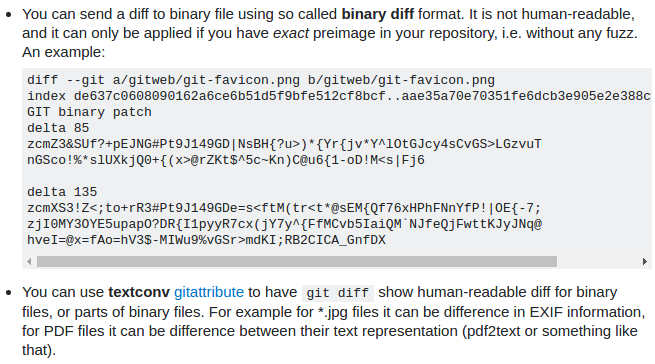
\includegraphics[scale=0.4]{GitWithBinary}
%  \caption{En illustration över över hur Git visar skillnader i binärfiler. Hämtat från stack overflow 2017-05-07.}
%  \label{fig:git_with_binary}
%\end{figure}
%\ \\
%Figur \ref{fig:git_with_binary} visar hur två olika versioner av en binärfil visas i Git. 
Skillnaden är helt oläslig för det mänskliga ögat och kräver att tilläggsprogram används för att antingen konvertera filen till ett textbaserat format eller översätta den till något begripligt. Ett exempel där användningen av ett sådan tilläggsprogram förklaras kan ses i bloggen \textit{Using Microsoft Word with Git} \cite{website:using_git_with_word}.

\subsection{Dokumentation med Molntjänster}
De två molntjänsterna som analyserades skiljer sig åt främst i en aspekt, Google Drive jobbar med WYSIWYG metodiken och ShareLaTeX jobbar med typsättning. Dokumentation för interna dokument var bland de tillfrågade personerna populärast med Google Drive. ShareLaTeX användes aldrig för dessa syften av samma anledning som togs upp i avsnitt \ref{subsec:wassing_documentation_by_wysiwyg}. 
\\ \\
Molntjänster hade den stora fördelen att de kördes i webbläsaren. Olika webbläsare producerade samma dokument med hjälp av tjänsten då tjänsten inte är beroende av vilken webbläsare som den körs i. Det gav fördelen att tekniska beroenden överfördes från lokal produktion till molntjänsten, som redan hade alla beroenden tillgodosedda.
\\ \\
Typsättning med molntjänster ansågs ha en nackdel. I stora dokument som innehöll flera underfiler kunde det bli jobbigt att kompilera och testa utseende på dokument när flera personer jobbade i filsystemet samtidigt. Icke färdigställda tabeller och skript kunde ge syntaxfel vid kompilering. Kolliderande beroenden för olika paket hade också varit ett problem. När den egna gruppen beslutade sig för att jobba med lokalt lagrade filer med versionshantering så var denna nackdelen huvudanledningen för att välja bort hantering via molntjänster. Ingen smidig lösning på det problemet stod att finna. Ett alternativ hade varit att duplicera dokumentarkivet för parallell testning, men det hade medfört andra problem.

\subsection{Kontrolläsning av dokument}
Kontrolläsning är inte ett dokumentationsverktyg, men en process som tar mycket tid vid dokumentationen. Det nämndes i intervjuerna att det hade varit önskvärt att ha ett verktyg eller åtminstone en procedur för att kontrolläsa bättre. Dock är kontrolläsning som arbetsmetod svårt att spika så att samma kvalitet på producerad text uppnås över hela dokumentationen, då människor kontrolläser olika. En sak som definitivt skulle vara nyttigt vore en utarbetad kontrolläsningsmetodik med punkter som behövde uppfyllas innan kontrolläsningen blev klar.
\\ \\
Den egna gruppen använde ett statusdokument på Google Drive för kontroll av producerade dokument. Detta statusdokument fylldes i bitvis med hittade fel och kommentarer på förbättringspotential. Statusdokumentet hanterades dåligt ansåg flera. Idén var god men användningen var inkonsekvent. Hur det här statusdokumentet hanterades borde ha varit en del av kontrolläsningsmetodiken.

\subsection{Lagring av dokument}
\label{subsec:wassing-document-storage}
Lokalt lagrade filer medförde problem. Ett väldigt stort tidsproblem var konfigurationen för att kunna jobba med lokalt lagrade filer. Gruppen behövde installera mjukvara för att kunna jobba med filerna lokalt, importera paket för att kunna använda funktioner och dessutom installera och använda samma kompilator. Kompilatorn som användes gav aldrig identiska resultat för hela gruppen, vilket kunde leda till olika utseende på kompilerade dokument för olika gruppmedlemmar. Detta hängde med som problem under hela projektet och resulterade i en del extrajobb för gruppens dokumentansvarig. 
\\ \\
Alternativet hade varit en uniform lösning, såsom ShareLaTeX. Mot projektets slut så tillfrågades den egna gruppens medlemmar om de inte hellre hade velat jobba med något annat verktyg. ShareLaTeX visade sig vara svaret hos några, då de ansåg att nackdelen att temporärt inte kunna kompilera för att flera personer arbetade i samma dokument eller att ha annorlunda versionshantering inte hade vägt tyngre än alla fördelar som ShareLaTeX medförde.

\subsection{Koordinering av arbetet}
\label{subsec:wassing-coordination-of-work}
En väsentlig del att ha i åtanke vid val av verktyg är koordineringsarbetet som gruppens dokumentansvarig behöver utföra. I den egna gruppen så användes en blandning av verktyg vilket gav dokumentansvarig en mängd saker att hålla koll på i form av utspridd dokumentation samt stöd för alla olika verktyg.
\\ \\
Det fanns bristande kunskap i LaTeX som ledde till att dokumentansvarig i början hjälpte flera medlemmar så att de kom igång med det faktiska skrivandet. Skrivandet blev dock inte försenat då dokumentansvarig lade all sin arbetstid på att hjälpa gruppen komma igång, men många arbetstimmar gick åt på det. Som tidigare nämnt i avsnitt \ref{subsec:wassing-document-storage} så hade en uniform lösning varit att föredra här för att minska startsträckan och tidsåtgången. 
En workshop eller föreläsning om användning av ett gemensamt verktyg samt konventioner i LaTeX hade mycket lättare kunna appliceras på en uniform plattform att jobba på.
\\ \\
Att gruppen använde en uniform mall för alla levererade dokument utom slutrapporten eliminerade många problem, såsom att dokumentets väsentligheter för att uppfylla kraven på struktur alltid fanns på samma ställe utan att enskilda skribenter behövde göra mycket. Det gjorde det lättare för dokumentansvarig att på en väldigt kort tidsperiod kunna bedöma att dokumenten kunde levereras. Mallen importerades alltid direkt i början av varje dokument som skrevs, vilket bara gick att uppnå med typsättning. Databasen för referenser användes dessutom av alla levererade dokument, även slutrapporten. Någon förbättringsmöjlighet sågs inte här.
\\ \\
Interna dokument som skrevs med hjälp av Google Drive blev väldigt varierande i utseende, men då de uppfyllde sina syften så ansågs utseendet inte vara av betydelse. Dokumentansvarig hade kunnat bestämma en tydligare struktur för var dokument lagrades på Drive. En struktur fanns men den efterföljdes inte alltid.
\\ \\
För en erfaren dokumentansvarig så hade det varit bra om även flera interna dokument hade skrivits i LaTeX. Det hade gått fort att sätta ihop dokumenten och de hade varit lätta att modifiera. Dessutom hade alla dokument fått ett enhetligt utseende och hade blivit lätta att navigera. Några dokument drog dock klar nytta av att de skrevs med Google Drive, såsom tidsrapporteringen. Tidsrapporteringen var fullpackad av funktioner som jobbade för att underlätta översikten för gruppens status i kursen. Sådana funktioner existerade inte i pdf-filer.
\\ \\
Det absolut viktigaste för dokumentansvarig är dock att varje användare kan jobba bra på egen hand med minimalt behov av hjälp. Lite extra koordineringsarbete är ingenting i jämförelse med att enskilda gruppmedlemmar behöver kontinuerlig hjälp med att skriva dokument. Därför bör valet av verktyg prioriteras utifrån vad medlemmarna känner sig bekväma med.

\subsection{Metod}
\label{sec:wassing-discussion-method}
Det finns en del faktorer som kan vara bra att nämna om undersökningens trovärdighet. Till att börja med så intervjuades enskilda personer beroende på om de hade tid och möjlighet. Dessa personer hade väldigt varierande roller i grupperna de jobbade med och alla var olika väl införstådda med hur deras respektive grupper jobbade med dokumentationen. Svaren som har insamlats under intervjuerna kan också vara vinklade beroende på tidigare erfarenheter med olika verktyg.
\\ \\
I avsnitt \ref{subsec:wassing-coordination-of-work} presenteras diskussionen utifrån författarens erfarenheter från projektet och diskussionen är därför vinklad.
\\ \\
I denna undersökning har ingen referens använts på hur intervjuerna skulle genomföras, utan frågorna som ställdes var endast resonerade utifrån vad författaren ville ha svar på. Detta i kombination med att författaren aldrig tidigare har gjort liknande intervjuer kan vara bra att ha i åtanke.

\section{Slutsatser}
\label{cha:wassing-conclusion}
%Vilka verktyg finns tillgängliga för att dokumentera i ett projektarbete och vilka uppenbara för- och nackdelar medför de?
%Vilka kriterier väger tyngst vid valet av verktyg att dokumentera med?
\subsection{Vilka verktyg finns tillgängliga för att dokumentera i ett projektarbete och vilka uppenbara för- och nackdelar medför de?}
Olika nivåer på kontrolläsning och utseende efter kompilering av filerna ledde till att några extra iterationer (versioner) på dokument behövde produceras. Skillnaderna i versionerna var små men felen behövde ändå åtgärdas. Versionerna på dokumenten hade blivit färre om det hade funnits en uniform standard. Allt utom kontrolläsningen hade åtgärdats om gruppen hade jobbat med ShareLaTeX, då ShareLaTeX som applikation redan är en editor, har alla paket och kompilerar på samma sätt oavsett vilken person som använder den eftersom den exekveras i webbläsaren.
\\ \\
Tillgängliga verktyg som användes av i princip alla grupper i olika omfång var WYSIWYG, både med och utan möjligheten att flera personer kan arbeta med ett dokument samtidigt samt typsättning, både med och utan versionshantering med lokalt eller globalt lagrade dokument. Studien har visat att för en grupp på sju till nio personer som sätts ihop slumpvis på Linköpings universitet i kursen TDDD96, där alla har blandade kompetenser, så är det bäst att enas någonstans i mitten vid verktygsvalet. Typsättning borde användas, men av den lättare graden att bara kod kan skrivas rakt av, utan förarbete. ShareLaTeX med full funktionalitet (premium) har visat sig medföra mest kvaliteter och minst problem när en grupp ställs inför de utmaningar som kursen erbjuder.

\subsection{Vilka kriterier väger tyngst vid valet av verktyg att dokumentera med?}
Tiden är den avgörande flaskhalsen när verktygen väljs. Tiden från det att gruppen börjar dokumentera tills det att dokumenten är färdiga är den aspekten som behöver minimeras, utan att kvaliteten ignoreras. Då ShareLaTeX kombinerar många verktyg till en hållbar grad och eliminerar många problem så anses frågan besvarad med att kriterierna inlärning, modularitet och kvalitet är viktigast. Dessa uppnås med hjälp av globalt lagrade dokument med typsättning och existerande stöd för olika plugins. Beroende på gruppens kompetens med typsättning och versionshantering i början av projektets start kan Git med lokalt lagrade filer användas för att uppnå bättre resultat i form av mer modularitet och bättre parallellt arbete. WYSIWYG bör i allmänhet undvikas för stora levererade dokument, speciellt om det är flera dokument som ska levereras.

%Killed footnotes, rip pretty document because unified standard...
%\footnote{Märkspråk är mer känt som Markup Language på engelska}
%\footnote{HTML är en förkortning av HyperText Markup Language}
%\footnote{Linux är ett operativsystem som Linus Torvalds publicerade 1991}
%\footnote{Mer känt som \textit{merge conflicts} på engelska, merge betyder sammanslagning}
%\footnote{Detta kallas på engelska \textit{WYSIWYG}, What you see is what you get}
%\footnote{Även känt som cache:ad data}
%Premiumkonto gick att uppnå på 2 olika sätt, antingen genom att betala för det eller genom att använda ShareLaTeXs inbjudningssystem\footnote{Mer känt som Referral-system på engelska} till att bjuda in ett antal andra personer att börja använda ShareLaTeX. 
%\footnote{Google Presentations är en del av Google Drive}
%\footnote{En plugin är en funktion som importerats externt för att utföra en eller flera uppgifter}
%\footnote{En editor är en mjukvara för att jobba med dokument}
%\footnote{Script är kodbitar som utför en eller flera funktioner}
%\footnote{Syntaxfel är ett fel som medför att en dator ej kan kompilera}